\chapter{Le CERFACS}
%\chapter{CERFACS : Le fondement des logiciels de simulation numérique}
%\chapter*{Le CERFACS : Le fondement des logiciels de simulation numérique}
%\addcontentsline{toc}{chapter}{Le CERFACS : Le fondement des logiciels de
                                %simulation numérique}

% Faire les sous parties

Le CERFACS est un laboratoire de recherche privé dont les actionnaires sont Airbus, le CNES (Centre National d'Études Spatiale), EDF (Électricité de France), Météo France, l'ONERA (Office National d'Études et de Recherche Aérospatiales), Safran et TotalEnergies. Il a pour but de développer la simulation numérique par le calcul HPC pour ses actionnaires, mais aussi de faire de la recherche et de former des ingénieurs, chercheurs et doctorants. Il a été créé en 1988 sous le statut de \ac{GIP}, pour devenir une société civile en 1996 et depuis 2021, le CERFACS est une SAS (Société par Actions Simplifiées).

\vspace{0,5cm}

Les deux bâtiments du CERFACS sont situés au Météopole, dans la partie Ouest de Toulouse. Environ 170 personnes y travaillent, dont 20 \% de femmes, 50\% de doctorants et 20\% d'étrangers dont la moitié ne sont pas Européens.

Physiciens, mathématiciens, informaticiens, numériciens et data Scientist y travaillent dans cinq équipes :

% Tout en français OU tout en anglais

\begin{itemize}
    \item \ac{ALGO-COOP}
    \item \ac{CSG}
    \item \ac{ES}
    \item \ac{AAM}
    \item \ac{GLOBC}
\end{itemize}

\hspace{0,5cm}

% (Algorithmes Parallèles \& sCientifics sOftware Operational Performances)
% (Équipe Informatique et Support Utilisateur)
% (Energy et Safety)
% (Advanced Aerodynamics and Multiphysics)
% (Modélisation du climat et de son changement global)

La \ac{CAO} permet de faire les plans numériques d'un avion par exemple, afin de s'assurer que toutes les pièces fabriquées vont bien s'imbriquer entre elles. Mais cela permet aussi de faire des simulations numériques pour prévoir à l'avance la tenue structurelle, les forces aérodynamiques, le volume sonore, etc. sans avoir à faire d'onéreux tests.

L'équipe AAM se focalise sur la simulation des écoulements en développant des méthodes numériques avancées et en les appliquant aux avions, fusées, hélicoptères, moteurs, turbomachines, etc. Les liens de l’équipe AAM avec toutes les autres équipes du CERFACS sont forts, car ces équipes utilisent aussi la \ac{CFD} de façon intensive pour prévoir leurs modèles : en effet, derrière ces thèmes, on retrouve en premier les équations qui régissent les écoulements des fluides.

\hspace{0,5cm}

Le CERFACS héberge des supercalculateurs (Kraken et Calypso) et un serveur sur lequel se trouve l'intranet avec toutes les ressources nécessaires aux employés.
Nous y trouvons notamment les liens vers la \ac{QVT}, le \ac{CSE}, un document "Plan du management de la qualité" et énormément d'autres ressources.
%Le \ac{CSSCT} et le \ac{DUERP} devraient obligatoirement y être présents selon le site du gouvernement. % détailler







\newpage

Après une recherche non fructueuse sur l'intranet, j'ai pu demander à la responsable de ressources humaines le document relatant des objectifs \ac{RSE}. Le document d'actions RSE est segmenté en trois parties principales :

\paragraph{Démarche RSE}

%En voici le contenu :

\begin{quote}
\setlength{\leftmargin}{0.5cm} % Ajuster la marge gauche
\setlength{\rightmargin}{0.5cm} % Ajuster la marge droite
    "Le Cerfacs n’a pas mis en place une démarche spécifique RSE mais des actions ont été réalisées dans
    ce cadre, vis-à-vis de l’écoresponsabilité, la qualité de vie au travail et une charte éthique a été
    incluse dans le règlement intérieur depuis décembre 2023 (intégrant notamment la prévention de la
    corruption et la gestion des conflits d’intérêts).
    \hspace{0,5cm}

    En outre, le Cerfacs achète ses fournitures auprès de créateurs solidaires (exemple : Antilope qui
    compte 32 salariés sur les 49 avec une reconnaissance de « travailleur handicapé »).
    \hspace{0,5cm}

    Le Cerfacs met à jour au moins deux fois par an et aussi souvent que nécessaire un document unique
    d’évaluation des risques Cerfacs (avec un plan d’actions de prévention).
    \hspace{0,5cm}

    Le Cerfacs a nommé des référents : un référent « Santé et Sécurité », un référent « \ac{RGPD} », un
    référent « Handicap », deux référents « Harcèlement, agissements sexistes et violences ».

    Un bilan HSE et RSE est présenté chaque année aux Associés du Cerfacs lors de l’Assemblée d’avril."
\end{quote}



\paragraph{Écoresponsabilité}
\hspace{0,5cm}

    J'ai constaté beaucoup d'actions dans le sens de l'écoresponsabilité lors de mon stage. La plupart sont mentionnées dans le document.
    \vspace{0,5cm}

    Un Groupe de Travail « Bilan carbone du CERFACS », composé de 10 volontaires, a été créé. Des bilans carbone ont été réalisés pour les années 2019 et 2021, en suivant la méthodologie proposée par le collectif de laboratoires Labos1point5\footnote{\url{https://labos1point5.org}}. Depuis mi-2023, le CERFACS collabore avec le Cabinet Take[air] pour établir un plan d’actions visant à réduire son empreinte carbone. Cette collaboration a permis de réaliser le bilan carbone de 2022 et de commencer l'élaboration d'un plan d'actions, qui devrait être finalisé à l’automne 2024, après la tenue de plusieurs ateliers. Finalement nous trouvons dans le document un tableau\ref{tab:Eco_actions} récapitulant les principaux postes d'émission identifiés dans une première colonne puis les objectifs et actions associés dans une seconde colonne.

    En parallèle, j'ai entendu parler de cette démarche en discutant avec des thésards. Et j'ai aussi pu trouver la page depuis l'intranet. Elle est divisée en cinq sections : "présentation", "actualités", émissions", "bilan" et "actions".
    J'aime beaucoup l'image ci-dessous, présente dans le document et le site internet, qui montre que le CERFACS réduit ses émissions d'année en année, probablement grâce aux efforts du groupe « Bilan carbone du CERFACS »  : 

    \begin{figure}[H]
        \centering
        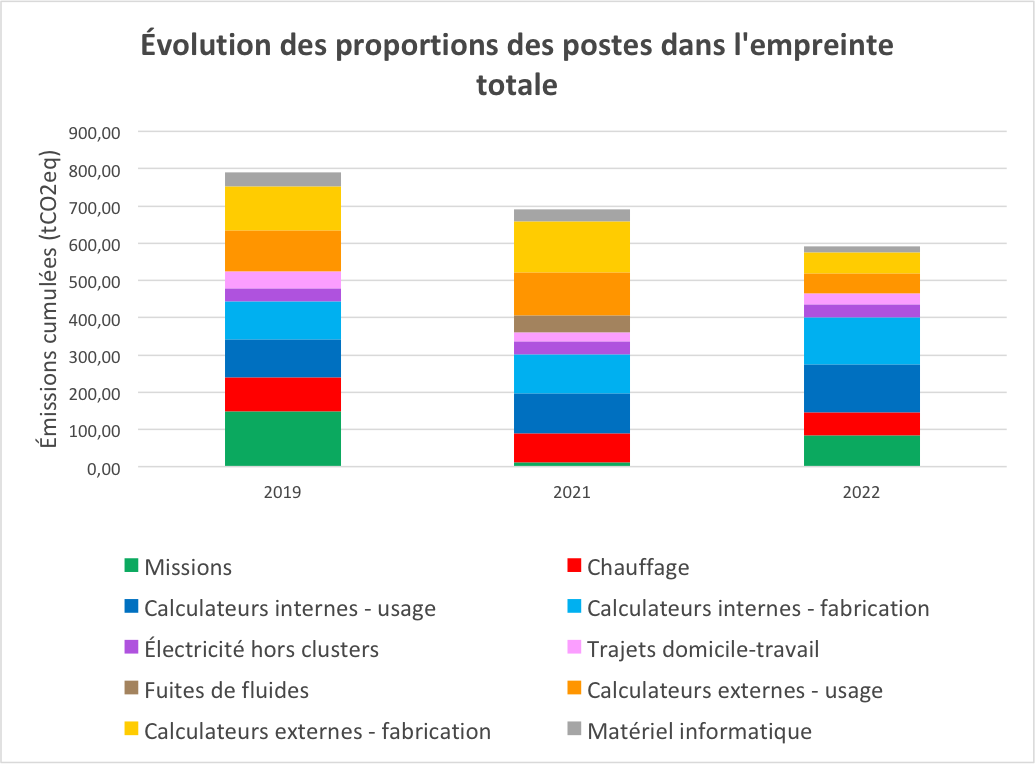
\includegraphics[width=0.85\textwidth]{images/evolution_postes_empreintecarbone.png}
        \caption{Evolution de l'empreinte carbone du CERFACS entre 2019 et 2022}
    \end{figure}

    Dans les couloirs du CERFACS on trouve des posters très clairs sur l'empreinte carbone d'un trajet pour une conférence en fonction des moyens de transports.

    Les employés sont incités à venir à vélo. Le CERFACS donne une prime pour chaque kilomètre fait à vélo sur le trajet habitation-travail-et vis-versa. Il y a aussi un atelier de réparation et des emplacements sécurisés pour les vélos.

    La politique de communication n'est pas spécialement tournée vers les efforts pour le climat ou la RSE, mais le CERFACS agit efficacement en ce sens.

\paragraph{Responsabilité sociale / Qualité de vie au travail}
\hspace{0,5cm}

    \begin{quote}
        \setlength{\leftmargin}{0.5cm} % Ajuster la marge gauche
        \setlength{\rightmargin}{0.5cm} % Ajuster la marge droite
        "La démarche Qualité de Vie au Travail (QVT) a été lancée au Cerfacs en janvier 2022, avec la mise en
        place d’un Groupe de Travail : elle a permis d’identifier 6 axes de travail pour améliorer le
        fonctionnement de la structure et du ressenti des personnes :
        \begin{itemize}
            \item Optimiser l’organisation et gestion du travail au niveau global
            \item Optimiser l’organisation et gestion du travail au niveau de l’équipe
            \item Optimiser l’organisation et gestion du travail au niveau personnel
            \item Assurer un meilleur accueil et support des non permanents
            \item Favoriser la vie sociale
            \item Améliorer le confort matériel"
        \end{itemize}
    \end{quote}

    De nouveau, un tableau\ref{tab:QVT_actions} détaille des exemples d'actions que j'ai pu experimenter (salle de repos, machine à café, endroit pour attacher son vélo, \dots)

    Un dernier plan d'action a été mis en place sur l'égalité professionnelle entre les femmes et les hommes. Il traite des sujets : l’embauche, la rémunération effective et l’articulation entre l’activité professionnelle et l’exercice de la responsabilité familiale.

    Je tiens à mentionner également que j'ai reçu un mail qui lançait un appel au volontariat pour composer le Comité de Pilotage pour la Prévention des Violences Sexistes et Sexuelles au Travail suite à une réunion d'information réalisée en collaboration avec la médecine du travail.

\newpage


Mon ressenti personnel sur le cadre de travail est très positif. Être assis dans un bureau climatisé avec une vue sur la campagne participe évidement à cela. Un des seuls risques à ce type de travail est une mauvaise position qui peut entraîner des problèmes de dos, épaules, etc. Pour palier cela il y a des affiches dans chaque bureau indiquant la meilleure position à avoir et proposant des exercices. Ces mêmes informations apparaissent dans le 'livret d'accueil stagiaire' qui m'a été remis le premier jour.

Une cantine présente sur le site à quelques minutes à pied, permet de déjeuner et échanger avec les collègues du CERFACS hors cadre professionnel.